% -*- latex -*-
%%%%%%%%%%%%%%%%%%%%%%%%%%%%%%%%%%%%%%%%%%%%%%%%%%%%%%%%%%%%%%%%
%%%%%%%%%%%%%%%%%%%%%%%%%%%%%%%%%%%%%%%%%%%%%%%%%%%%%%%%%%%%%%%%
%%%%
%%%% This text file is part of the source of 
%%%% `Parallel Computing'
%%%% by Victor Eijkhout, copyright 2012/3
%%%%
%%%%%%%%%%%%%%%%%%%%%%%%%%%%%%%%%%%%%%%%%%%%%%%%%%%%%%%%%%%%%%%%
%%%%%%%%%%%%%%%%%%%%%%%%%%%%%%%%%%%%%%%%%%%%%%%%%%%%%%%%%%%%%%%%

\Level 0 {Basics}

\Level 1 {The OpenMP model}

OpenMP has has a model, that is, an abstract way of thinking
about program execution,
that is based on \indexterm{threads}. (For more on threads, 
see \HPSCref{sec:threads}.) At the start of your program, 
there is typically some sequential work, and that gets executed
by a single thread, the \emph{master thread}\index{threads!master}. Then,
when the opportunity for parallelism offers itself, 
\indextermsub{worker}{threads} can come into action.

Of course, OpenMP is not magic, so you have to tell it when something
can be done in parallel. This is done through \indexterm{directives}
that precede a block of parallelizable code. Here is a very simple example:
\verbatimsnippet{hello-omp}
It prints out the `hello world' message once for each thread. How many
threads there are is controlled outside of your program.

The way you should view this is as follows.
\begin{itemize}
\item Immediately preceding the parallel block, one thread will be
  executing the code. Typically this is the
  \indextermsub{master}{thread}.
\item At the start of the block, a new \indextermbus{thread}{team} is
  created; this includes the thread that was active before the block.
\item Each thread in the team then executes the body of the block; it
  will have access to all variables of the surrounding environment.
\end{itemize}
This is illustrated in figure~\ref{fig:fork-join} below.

\Level 1 {Some context}

\Level 2 {OpenMP code structure}
\commandref{omp-code}

OpenMP is largely based on directives: instructions to the compiler
and runtime that are hidden in comment-like structures. In Fortran,
the directives are actually in a comment:
\begin{verbatim}
!$OMP construct
\end{verbatim}
while in C they are hidden in a \indexterm{pragma}: something that
is normally meant for the \indextermbus{C}{preprocessor}:
\begin{verbatim}
#pragma omp construct
\end{verbatim}
After the directive, in~C you usually find a `structured block':
a single statement or a block in curly braces. In~Fortran,
the directive is explicitly closed with
\begin{verbatim}
!$OMP END construct
\end{verbatim}

There are also a couple of OpenMP routines, and for that
you need to include
\begin{verbatim}
#include "omp.h"
\end{verbatim}
in C, and 
\begin{verbatim}
use omp_lib
\end{verbatim}
for Fortran.

\Level 2 {Compiling}

OpenMP is handled by extensions to your regular compiler, typically by
adding an option to your commandline:
\begin{verbatim}
# gcc
gcc -o foo foo.c -fopenmp
# Intel compiler
icc -o foo foo.c -openmp
\end{verbatim}
If you have separate compile and link stages, you need that option in both.

When you use the openmp compiler option, a \indexterm{cpp} variable \indextermtt{_OPENMP}
will be defined. Thus, you can have conditional compilation by writing
\begin{verbatim}
#ifdef _OPENMP
   ...
#else
   ...
#endif
\end{verbatim}

\Level 2 {Running an OpenMP program}

You run an OpenMP program by invoking it the regular way (for instance \n{./a.out}),
but its behaviour is influenced by some \indextermbus{OpenMP}{environment variables}.
The most important one is \indextermtt{OMP_NUM_THREADS}:
\begin{verbatim}
export OMP_NUM_THREADS=8
\end{verbatim}
which sets the number of threads that a program will use.

\Level 0 {Background on threads}

When an OpenMP program starts, on the \indextermsub{master}{thread} 
is active.
OpenMP directives create parallel regions
\begin{figure}[ht]
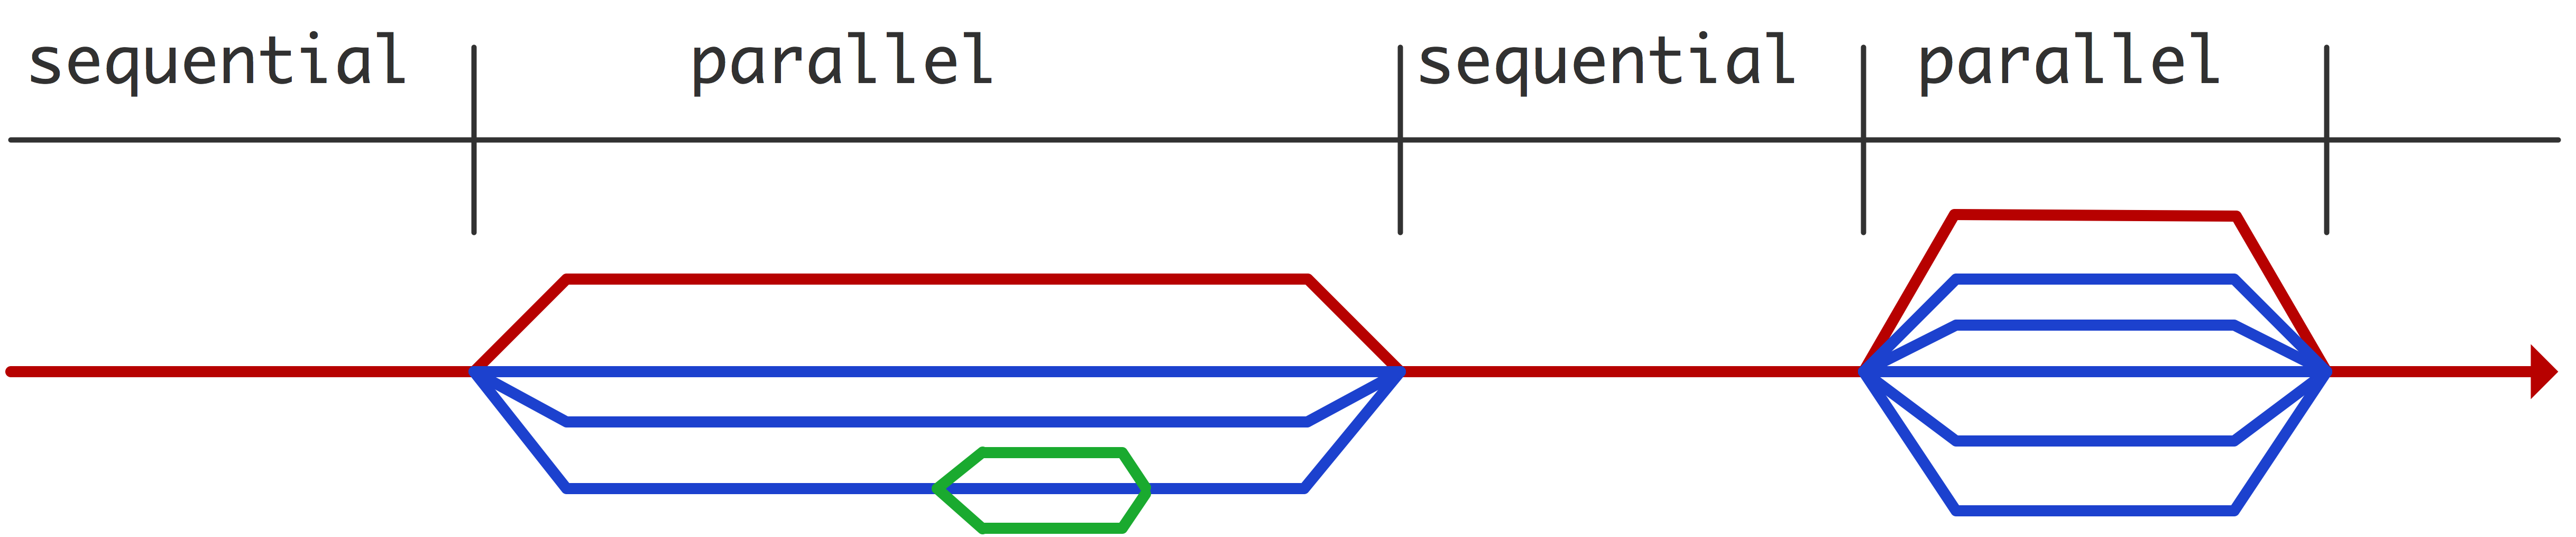
\includegraphics[scale=.08]{fork-join}
\caption{Thread creation and deletion during parallel execution}
\label{fig:forkjoin}
\end{figure}
in which a \indextermbus{thread}{team} is active. 
The thread team can be spawned by the master thread,
or recursively by another thread. This is illustrated
in figure~\ref{fig:forkjoin}.

\Level 1 {Parallel regions}
\commandref{omp-parallel}

The simplest way to create a parallel region is through the 
\indexpragma{parallel} pragma. In~C this is followed by a block,
in Fortran you conclude the block with \texttt{end parallel}.
\begin{verbatim}
#pragma omp parallel
{
  // this is executed by all threads
}
\end{verbatim}
It would be pointless to have the block be executed identically by
all threads, so you will probably use the functions
\indextermtt{omp_get_thread_num}, to find out which thread you are, and
\indextermtt{omp_get_num_threads}, to find out the total number of threads.
Both these functions give a number relative to the current team;
recall from figure~\ref{fig:forkjoin} that new teams can be created recursively.

\begin{exercise}
  What happens if you call \n{omp_get_thread_num} and \n{omp_get_num_threads}
  outside a parallel region?
\end{exercise}

\Level 1 {Thread data}
\commandref{sec:ompdata}

A thread has access to variables of two kinds. Variables on the
\indexterm{heap} are typically created by a call to \indextermtt{malloc}
(in~C) or \indextermtt{new} (in~C++). Threads that are spawned have
the same type of access to them.

There are also variables on the \indexterm{stack}, which have a local
\indexterm{scope}. Thread access to such variables is more complicated,
since each thread has its own \indexterm{context}. Most relevant to our story,
the context can contain local copies of variables, that is, each thread
has a variable, say~\n{x}, but they are local to each thread context.
Thus, one thread setting its~\n{x} has no influence on what
another thread sees as the value of its~\n{x}.

To use the technical term, there are
\begin{itemize}
\item \indexterm{shared variables},
  where each thread refers to the same data item, and 
\item \indexterm{private variables},
  where each thread has its own instance.
\end{itemize}
%
\begin{figure}[ht]
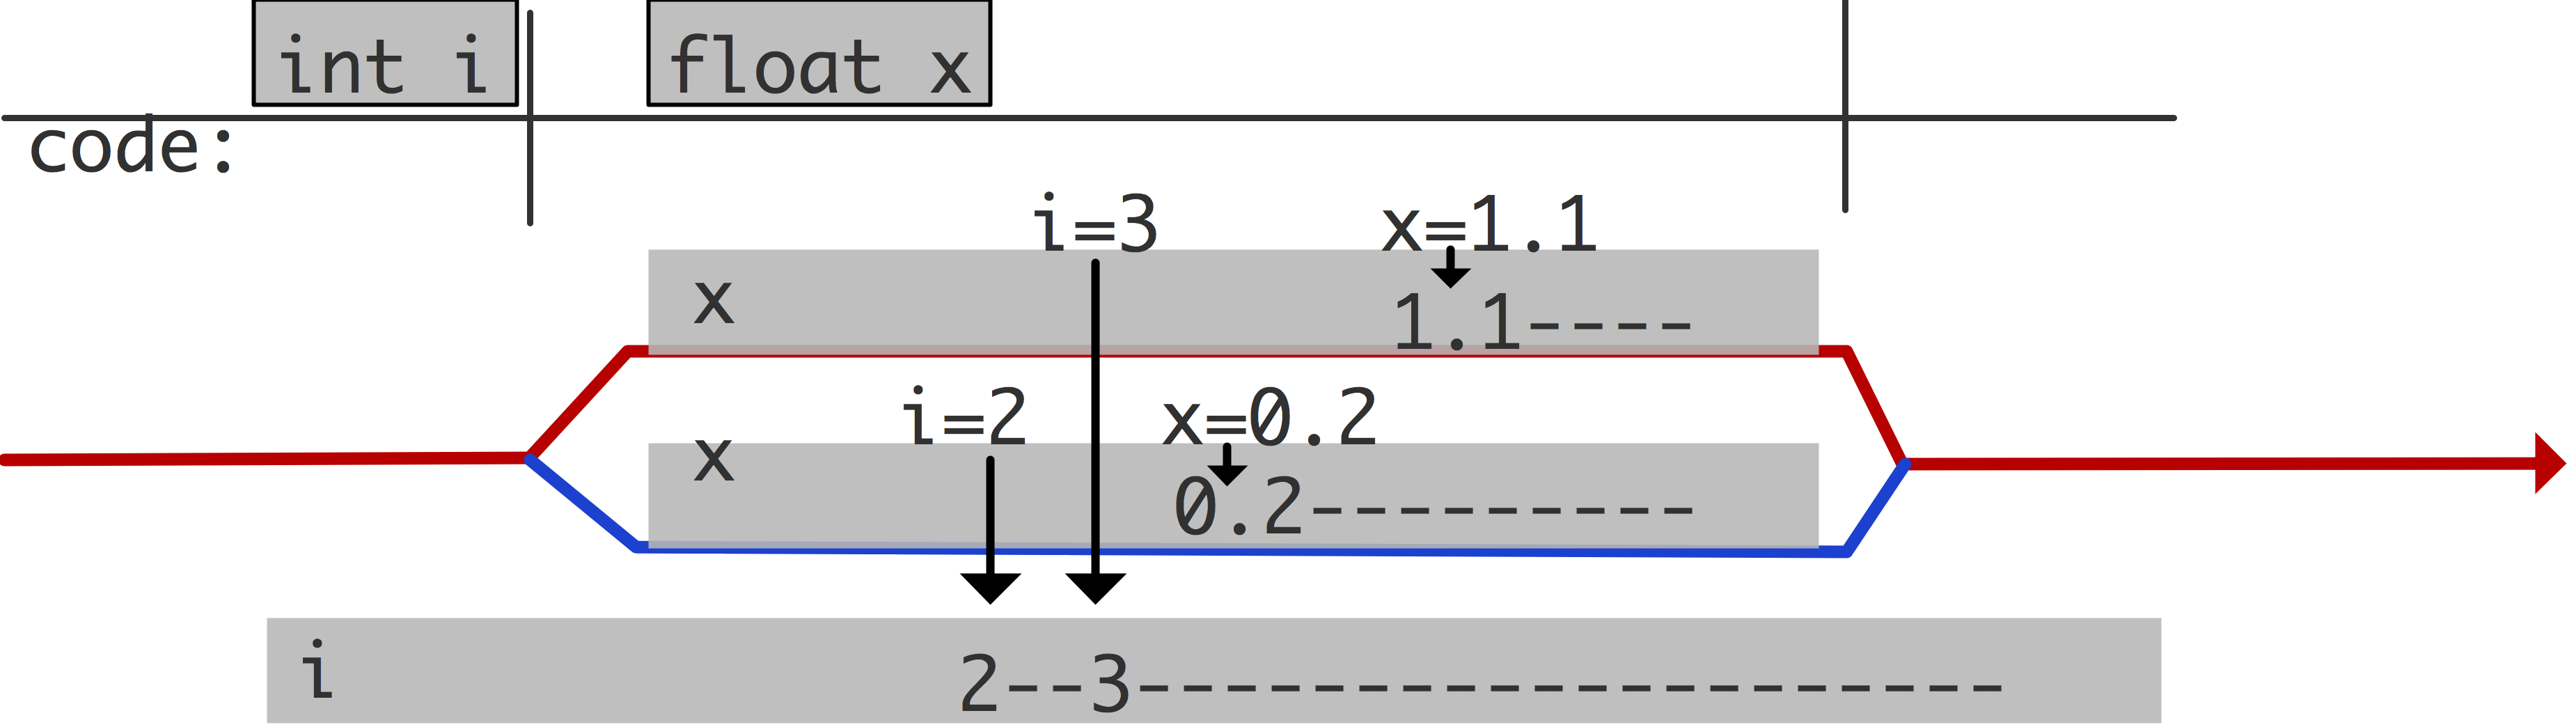
\includegraphics[scale=.1]{fork-join-vars}
\caption{Locality of variables in threads}
\label{fig:threadvars}
\end{figure}
%
This is illustrated in figure~\ref{fig:threadvars}.

When a new \emph{thread team}\index{thread!team!and variable access} is created,
there are various mechanisms for indicating which variables are shared
and which are private.
\begin{itemize}
\item Any variable declared inside the parallel region is private. In
  the following code segment the variable~\n{x} is local to the
  thread: the value that is set by one thread does not interfere with
  what other threads do.
\begin{verbatim}
#omp parallel
{
  double x;
  x = // some dynamic value
  ... = .... x ....
}
\end{verbatim}
\item By default, any variable declared in the surrounding scope is
  shared. Thus, in the following code segment, each thread sets the
  value of~\n{x}, and its value after the parallel region is
  indeterminate.
\begin{verbatim}
int x;
#omp parallel
{
  x = omp_get_thread_num();
}
// what is the value of x?
\end{verbatim}
\item In a parallel loop, the loop variable is private, even though it may
  have been declared outside the parallel construct.
\item A variable declared in the surrounding scope can explicitly be
  declared private or shared by adding a \indexpragma{private}
  or \indexpragma{shared} clause respectively to the OpenMP
  directive. In the following fragment, each 
  For the behaviour of shared variables, the default, see the point above.
\item Unless otherwise stated, private variables are undefined at the
  start of the parallel region, and disappear at the end; shared
  variables become undefined after the parallel region.
\item Data allocated on the \indexterm{heap} is
  shared\footnote{However, note that the C~and~Fortran standards do
    not actually define a~heap. Therefore it is wise to spell out your
    intentions.}.
\end{itemize}

\Level 0 {Controlling thread data}

\Level 1 {Private data}
\commandref{omp-private}

The \indexpragma{private} directive declares data to have a separate copy 
in the memory of each thread. By default, such private variables are uninitialized
at the begin of the parallel region, and any computed value goes away at the end 
of the parallel region. You can force initialization with \indexclause{firstprivate},
and preserving the last iteration with \indexclause{lastprivate}.

Private arrays are tricky.
\begin{itemize}
\item In C, if an array is statically defined, e.g.,
\begin{verbatim}
double a[2][5];
\end{verbatim}
declaring \n{private(a)} will indeed put a copy on in each thread.
Note that this will lead to an explosion in memory use; in fact, for large arrays you
  may experience \indextermbus{stack}{overflow}.
\item Dynamically allocated arrays, e.g.,
\begin{verbatim}
double *a; a = (double*) malloc( some_size );
\end{verbatim}
can not be private with \n{private(a)}: this only gives each thread 
a private pointer, but these pointers all point to the same memory location.
\end{itemize}

\Level 1 {Default}

As remarked, most data in a parallel section is shared. This default behaviour can be 
controlled by adding a \indexpragma{default} clause:
\begin{verbatim}
#pragma omp parallel default(shared) private(x)
{ ... }
#pragma omp parallel default(private) shared(matrix)
{ ... }
\end{verbatim}
and if you want to play it safe:
\begin{verbatim}
#pragma omp parallel default(none) private(x) shared(matrix)
{ ... }
\end{verbatim}

\Level 0 {Parallel regions}
\commandref{parallelregion}

The simplest way to create parallelism in OpenMP is to use
the \indexpragma{parallel} pragma. A~block preceded by the \n{omp parallel} pragma
is executed by a newly created team of threads. 
This is an instance of the \indexac{SPMD} model: all threads execute the same
segment of code.
Since it would not be interesting to have all threads do the same calculations,
you can use the function \indexcommand{omp_get_thread_num} to distinguish 
between them.

For instance, if you program computes
\begin{verbatim}
result = f(x)+g(x)+h(x)
\end{verbatim}
you could parallelize this as
\begin{verbatim}
double result = 0;
#pragma omp parallel
{
  int num = omp_get_thread_num();
  if (num==0)      result += f(x);
  else if (num==1) result += g(x);
  else if (num==2) result += h(x);
}
\end{verbatim}
This example shows how the three functions are computed in parallel,
but other than that \textbf{there are many things wrong with this example}.
The rest of this section will be about explaining what is wrong here,
and what can be done about it.

\Level 1 {Thread data in parallel regions}

Private variables act as is they are created at the start of the parallel region.
Sometimes it may be desirable to have them initialized with their prior value;
the clause \indexpragma{firstprivate} initializes them with the value of the
surrounding scope. (The \indexpragma{copyin} directive does more or less the same thing.)
\begin{verbatim}
double x;
x = .... // initial value
#omp parallel firstprivate(x)
{
  ... = .... x .... // still the initial value
}
\end{verbatim}

Private variables also disappear at the end of the parallel region. 
If you want to preserve the value of a private variable, for instance
because it computed something interesting, you need to indicate that.
A~common case is preserving the result of the last iteration of a parallel loop
which is done with \indexpragma{lastprivate}
\begin{verbatim}
double x;
#omp parallel for lastprivate(x)
for (...) {
    x = ....
}
// now x has the value computed in the last iteration
\end{verbatim}

\Level 0 {Work sharing}

The parallel regions of section~\ref{sec:parallelregion} were a case of \ac{SPMD} programming,
where the same code gets executed by all workers. In contrast to this, OpenMP has \indexterm{work sharing}
constructs, where the work is split up between the threads.

\Level 1 {Loop parallelism}
\commandref{omp-for}

The parallel execution of a loop can be handled a number of different ways.
For instance, you can create a parallel region around the loop, and
adjust the loop bounds:
\begin{verbatim}
#pragma omp parallel
{
  int threadnum = omp_get_thread_num(),
    numthreads = omp_get_num_threads();
  int low = N*threadnum/numthreads,
    high = N*(threadnum+1)/numthreads;
  for (i=low; i<high; i++)
    // do something with i
}
\end{verbatim}

A more natural option is to use the
\indexpragma{parallel for} pragma:
\begin{verbatim}
#pragma omp parallel for
for (i=0; i<N; i++) {
  // do something with i
}
\end{verbatim}
This has several advantages. For one, you don't have to calculate the loop bounds
for the threads yourself, but you can also tell OpenMP to assign the loop
iterations according to different schedules.

Using \n{parallel for} is actually short hand for using a \n{parallel} pragma,
which creates the threads, and inside a \n{for} pragma, which spreads the loop 
iterations over the thread team that encounters the loop. The \n{for} pragma
does not create threads itself.

The loop has to satisfy a number of basic constraints, such as that you can not
jump out of it.

\Level 2 {Loop schedules}

Usually you will have many more iterations in a loop than there are threads.
Thus, there are several ways you can assign your loop iterations to the threads.
OpenMP lets you specify this with the \indextermtt{schedule} clause.
\begin{verbatim}
#pragma omp for schedule(....)
\end{verbatim}

The first distinction we now have to make is between static and dynamic schedules.
With static schedules, the iterations are assigned purely based on the number
of iterations and the number of threads (and the \n{chunk} parameter; see later).
In dynamic schedules, on the other hand, iterations are assigned to threads that
are unoccupied. Dynamic schedules are a good idea if iterations take an unpredictable
amount of time, so that \indexterm{load balancing} is needed.

The default static schedule is to assign one consecutive block of iterations
to each thread. If you want different sized blocks you can defined a \indexclauseoption{schedule}{chunk} size:
\begin{verbatim}
#omp pragma for schedule(static[,chunk])
\end{verbatim}
(where the square brackets indicate an optional argument).
With static scheduling, the compiler will split up the loop iterations at compile time,
so, provided the iterations take roughly the same amount of time, this is the most efficient at runtime.

The choice of a chunk size is often a balance between the low overhead of having 
only a few chunks, versus the load balancing effect of having smaller chunks.
\begin{exercise}
  Why is a chunk size of~1 typically a bad idea? (Hint: think about
  cache lines, and read \HPSCref{sec:falseshare}.)
\end{exercise}

In dynamic scheduling OpenMP will put blocks of iterations
(the default chunk size is~1) in a task queue, and the threads take one of these
tasks whenever they are finished with the previous.
\begin{verbatim}
#omp pragma for schedule(static[,chunk])
\end{verbatim}
While this schedule may give good load balancing if the iterations
take very differing amounts of time to execute, it does carry runtime
overhead for managing the queue of iteration tasks.

Finally, there is the \indexclauseoption{schedule}{guided} schedule, which gradually decreases the chunk size.
The thinking here is that large chunks carry the least overhead, but smaller chunks are better
for load balancing.

If you don't want to decide on a schedule in your code, you can
specify the \indexclauseoption{schedule}{runtime} schedule. The actual
schedule will then at runtime be read from the
\indextermtt{OMP_SCHEDULE} environment variable. You can even just
leave it to the runtime library by specifying
\indexclauseoption{schedule}{auto}

\Level 2 {While loops}

OpenMP can only handle `for' loops: \indexterm{while loops} can not
be parallelized. So you have to find a way around that. While loops
are for instance used to search through data:
\begin{verbatim}
while ( a[i]!=0 && i<imax ) {
 i++; }
// now i is the first index for which \n{a[i]} is zero.
\end{verbatim}
We replace the while loop by a for loop that examines all locations:
\begin{verbatim}
result = -1;
#omp parallel for
for (i=0; i<imax; i++) {
  if (a[i]!=0 && result<0) result = i;
}
\end{verbatim}
\begin{exercise}
  Show that this code has a race condition.
\end{exercise}
You can fix the race condition by making the condition into a critical section;
section~\ref{sec:critical}. In this particular example, with a very small amount
of work per iteration, that is likely to be inefficient 
in this case (why?).
A~more efficient solution uses the \indexpragma{lastprivate} pragma:
\begin{verbatim}
result = -1;
#omp parallel for lastprivate(result)
for (i=0; i<imax; i++) {
  if (a[i]!=0) result = i;
}
\end{verbatim}
You have now solved a slightly different problem: the result variable
contains the \emph{last} location where \n{a[i]} is zero.

\Level 1 {Sections}

\Level 1 {Single/master}

\indexpragma{master}
\indexpragma{single}

These pragmas can for instance be used to print tracing information.
\begin{verbatim}
#pragma omp parallel
{
#pragma omp single
  printf("We are starting this section!\n");
  // parallel stuff
}
\end{verbatim}

\Level 0 {Reductions}
\commandref{reduction}

Parallel tasks often produce some quantity that needs to be summed
or otherwise combined.
In section~\ref{sec:parallelregion} you saw an example, and it was stated that the
solution given there was not very good.

The problem in that example was the race condition involving the \n{result}
variable. The simplest solution is to eliminate the race condition
by declaring a \indexterm{critical section}:
\begin{verbatim}
double result = 0;
#pragma omp parallel
{
  double local_result;
  int num = omp_get_thread_num();
  if (num==0)      local_result = f(x);
  else if (num==1) local_result = g(x);
  else if (num==2) local_result = h(x);
#pragma omp critical
  result += local_result;
}
\end{verbatim}

This is a good solution if the amount of serialization in the critical section
is small compared to computing the functions~$f,g,h$. On the other hand, you
may not want to do that in a loop:
\begin{verbatim}
double result = 0;
#pragma omp parallel
{
  double local_result;
#pragma omp for
  for (i=0; i<N; i++) {
    local_result = f(x,i);
#pragma omp critical
    result += local_result;
  } // end of for loop
}
\end{verbatim}
\begin{exercise}
  Can you think of a small modification of this code, that still uses a critical section,
  that is more efficient? Time both codes.
\end{exercise}

Another strategy would be to
`duplicate' the global variable and gather the contributions later:
\begin{verbatim}
double result,local_results[3];
#pragma omp parallel
{
  int num = omp_get_thread_num();
  if (num==0)      local_results[num] = f(x)
  else if (num==1) local_results[num] = g(x)
  else if (num==2) local_results[num] = h(x)
}
result = local_results[0]+local_results[1]+local_results[2]
\end{verbatim}
and this may work if you are just dealing with a few function invocates. 
However, If you use local results for a parallel loop beware of \indexterm{false sharing}; 
see \HPSCref{sec:falseshare} for an explanation.

The easiest way to effect a reduction is of course to the use the \indextermtt{reduction}
clause. Adding this to an \n{omp for} loop has the following effect:
\begin{itemize}
\item OpenMP will make a copy of the reduction variable per thread,
  initialized to the identity of the reduction operator, for instance
  $1$~for multiplication.
\item Each thread will then reduce into its local variable;
\item At the end of the loop, the local results are combined, again
  using the reduction operator, into the global variable.
\end{itemize}
This is one of those cases where the parallel execution can have a slightly different
value from the one that is computed sequentially, because floating point operations
are not associative. See~\HPSCref{sec:roundoff-parallel} for more explanation.

\Level 0 {Synchronization}

In the constructs for declaring parallel regions above, you had little control over 
in what order threads executed the work they were assigned.
This section will discuss \indexterm{synchronization} constructs: ways of telling
threads to bring a certain order to the sequence in which they do things.

\Level 1 {Barrier}
\commandref{exbarrier}

A barrier defines a point in the code where all active threads will stop
until all threads have arrived at that point. With this, you can guarantee that
certain calculations are finished. For instance, in this code snippet, computation 
of~\n{y} can not proceed until another thread has computed its value of~\n{x}.
\begin{verbatim}
#pragma omp parallel 
{
  int mytid = omp_get_thread_num();
  x[mytid] = some_calculation();
  y[mytid] = x[mytid]+x[mytid+1];
}
\end{verbatim}
This can be guaranteed with a \indexpragma{barrier} pragma:
\begin{verbatim}
#omp parallel 
{
  int mytid = omp_get_thread_num();
  x[mytid] = some_calculation();
#pragma omp barrier
  y[mytid] = x[mytid]+x[mytid+1];
}
\end{verbatim}

\Level 1 {Mutual exclusion: \texttt{critical} and \texttt{atomic}}
\commandref{critical}

Sometimes it is necessary to let only one thread execute a piece of code.
Such a piece of code is called a \indexterm{critical section}, and
there are two pragmas for critical sections: \indexpragma{critical} and \indexpragma{atomic}.
The second one is more limited but has performance advantages.

The most common use of critical sections is to update a variable. Since updating
involves reading the old value, and writing back the new, this has the possibility
for a \indexterm{race condition}: another thread reads the current value
before the first can update it; the second thread the updates to the wrong value.

Thus:
\begin{verbatim}
#pragma omp paralle
{
  int mytid = omp_get_thread_num();
  double tmp = some_function();
#pragma omp critical
  sum += tmp;
}
\end{verbatim}

A \n{critical} section works by acquiring a lock, which carries a substantial overhead.
Furthermore, if your code has multiple critical sections, they are all mutually exclusive:
if a thread is in one critical section, the other ones are all blocked.

On the other hand, the syntax for \n{atomic} sections is limited, but such sections
are not exclusive and they can be more efficient, since they assume that there is a hardware
mechanism for making them critical.

The problem with \n{critical} sections being mutually exclusive can be mitigated by naming them:
\begin{verbatim}
#pragma omp critical (optional_name_in_parens)
\end{verbatim}

\Level 1 {Locks}

OpenMP also has the traditional mechanism of a \indexterm{lock}. A~lock is somewhat similar to 
a critical section: it guarantees that some instructions can only be performed by one
process at a time. However, a critical section is indeed about code; a~lock is about data.
With a lock you make sure that some data elements can only be touched by one process at a time.

One simple example of the use of locks is generation of a \indexterm{histogram}.
A~histogram consists of a number of bins, that get updated depending on some data.
Here is the basic structure of such a code:
\begin{verbatim}
int count[100];
float x = some_function();
int ix = (int)x;
if (ix>=100)
  error();
else
  count[ix]++;
\end{verbatim}
It would be possible to guard the last line:
\begin{verbatim}
#pragma omp critical
  count[ix]++;
\end{verbatim}
but that is unnecessarily restrictive. If there are enough bins in the
histogram, and if the \n{some_function} takes enough time, there are unlikely to be
conflicting writes. The solution then is to create an array of locks, with
one lock for each \n{count} location.

\Level 0 {Dependency analysis}

\Level 1 {Anti/output dependencies}

\begin{verbatim}
for (i=0; i<N-1; i++) 
  A[i] = A[i+1]
\end{verbatim}
becomes
\begin{verbatim}
for (i=0; i<N-1; i++) 
  tmp[i] = A[i+1]
for (i=0; i<N-1; i++) 
  A[i] = tmp[i]
\end{verbatim}
which can be individually parallelized.

\Level 0 {Stuff}

\Level 1 {Timing}
